\documentclass{article}
\usepackage{epstopdf}
\usepackage{graphics}
\usepackage{graphicx}
\usepackage{amsmath}

\usepackage{tikz}
\usepackage{listings}
\usepackage{csvsimple}
\usepackage{nicefrac}
\usepackage{units}

\linespread{1.6}

\title{Project II: Big Brother is Watching You!}
\date{2015-11-02}
\author{Albert Quizon, Christopher Silvia, Siyu Yang}
\begin{document}

\maketitle
\newpage


\section{Instructions}
\section{Model Assumptions}
\section{Parameter Values and their Justifications}
\subsection {Gotham City}
As the original construction in the Batman Series, Gotham City is New York City Mahattan area below 14th Street. For simplicity, we are assuming that Gotham City is a 3 miles – by – 3 miles square area. Gotham University (a fictional depiction of NYU) and the Financial District are reduced respectively to a $0.5 \times 0.5$ and a $1 \times 1$ square miles square areas. Assume the two areas are seperate.
\subsection{Technical Data for UAV}
***insert other stuff***
Speed of UAV is considered 16 meters per second.
\subsection{Ground Sampling Distance}
The work \textit{Drones And Aerial Observation} introduced an equation regarding Ground Sampling Distance (GSD) – the area a drone will be able to observe at a given cruise height:
\begin{equation}
GSD = \frac{\text{pixel size x height above ground level}}{\text{focal length}}
\end{equation}
If we assume that the drone is armed with Canon S100, a most common filming device used by UAVs, we will have a camera with pixel size of 0.0019mm, focal length ranging from 24 – 120mm, and can produce images of up to 4,000 by 4,000 pixels. Assuming a cruise height of 1000 meters, we will be able to get a 1000 ft by 1000 ft surveillance vision every given moment.
\section {Simulation Algorithm}
\subsection {Model I: Rectangular Patrol Path}
For the first simple discrete model, we are going to estimate where every single drone would cover a given square area on the map. For any given drone, it will be patrolling a given rectangular area. We need to make sure in the interval of 15 minutes (900 seconds), the drone will cover the whole area. Thus we are considering a 304.8 meter (1000 feet) wide "snake" drawing out a rectangular region for all 15 minutes, with ground speed 16 meters per second (35.71 miles per hour). This would cover:
\begin{equation}
35.71 \unitfrac{mi}{hr} \times 15 minute \times 1000 feet = 1.7 miles^2
\end{equation}
To cover all of Gotham City (assumed as a 4828 by 4828 meters$^{2}$ square = 23,309,584 $[m^{2}]$) in 15 minutes, we need at least 6 drones ($\frac{23309584}{4389120} = 5.31$).  

In order to increase patroling around Gotham University and Financial district to every 5 minutes, and the rest of the area every 20 minutes, we have the designated patrol area of every drone around critical region:
\begin{equation}
35.71 \unitfrac{mi}{hr} \times 5 minute \times 1000 feet = 0.6 miles^2
\end{equation}
and patrol area of every drone around none-critical region:
\begin{equation}
35.71 \unitfrac{mi}{hr} \times 20 minute \times 1000 feet = 2.5 miles^2
\end{equation}

Which means we need 1 drone to continuously patrol the $0.25$ square miles of region around Gotham University, and 2 drones to patrol the area around Financial district. For the rest of area, we would need 3 other drones to cover. We can easily implement the need for refueling every 5 hours by providing another set of 6 drones which will take over for the first set of drones while they recharge. We make the assumption that drones can recharge/refuel in under 5 hours. This means the city needs at least 12 drones to monitor that no point in the city goes unobserved for more than 15 minutes in a row. 

We can see that the above model is very crude and limited. It assumes that the drones would draw out $9 miles \times 1000 feet $ rectangles on the map for 15 minutes, without considering refueling, turns and cost. Areas around Gotham University and Financial districts are over patrolled, resulting in higher cost. Moreover, the patrol routes are fixed, resulting in no randomness and thus could easily calculate a jaywalk route without getting caught. Based on the weaknesses above, we present the second model.


\subsection {Model II: Ideal Gas Model}
The second model we present is a Ideal Gas Model were drones fly on random directions in uniform speed. When a drone reaches the boundary of the surveillance region, that drone``bounces off'' (see Figure \ref{fig:drone-barrier-bounce}).
Note that if the wall is vertical, the bouncing just multiplies the $x$ component of the velocity by $-1$.

\begin{figure}[h]
\begin{center}
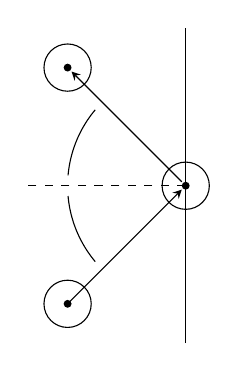
\begin{tikzpicture}

% wall/boundary for drone to bounce off of
\draw (1,-2) to (1,2);

% drone before bounce
\draw (-0.5,-1.5) circle (0.3);
\fill (-0.5,-1.5) circle [radius=0.05];

% drone during bounce
\draw (1.0, 0.0) circle (0.3);
\fill (1.0, 0.0) circle [radius=0.05];

% drone after bounce
\draw (-0.5, 1.5) circle (0.3);
\fill (-0.5, 1.5) circle (0.05);

% bouncing arrows
\draw[->,>=stealth] (-0.5, -1.5) -- (0.95,-0.05);
\draw[->,>=stealth] (0.95, 0.05) -- (-0.45, 1.45);

% line of symmetry
\draw[dashed] (1,0) to (-1,0);

% angle measures
\draw[domain=140:175] plot ({1 + 1.5*cos(\x)}, {1.5*sin(\x)});
\draw[domain=-175:-140] plot ({1 + 1.5*cos(\x)}, {1.5*sin(\x)});

\end{tikzpicture}
\end{center}
\caption{An incoming drone bounces off of a barrier.  The circle is its radius
	of vision.}
\label{fig:drone-barrier-bounce}
\end{figure}


If the drones do not interact with each other, and are given uniformly random velocities and positions, then they should be distributed uniformly throughout the surveillence domain.

We have implemented a simulation of this model in matlab.
A typical moment in time looks like this:

\begin{figure}[h]
\begin{center}
\begin{tikzpicture}
\end{tikzpicture}
\end{center}
\end{figure}

Notice that in this case, the drones' fields of view are overlapping.

\section{Code Appendix}
\lstinputlisting[language=octave,
	caption={Ideal Gas Simulation}, 
	label=code:ideal-gas]
{ideal-gas.m}

\section{Model Predictions}
\section{Validation}
\section{Strengths and Weakness}
\section{Future Work}
\section{Conclusions}
\section{references}

\end{document}
